%!TEX root = index.tex
\chapter{Introduction to Air Traffic Management}

This chapter will provide basic introduction to the field of ATM (Air Traffic Management), starting with brief summary of the history of aviation and continuing with explanation of some basic terms and concepts that will be needed further.

The Air Traffic Management is an umbrella term for three services provided in aviation: Air Traffic Control (ATC), Air Traffic Flow Management (ATFM) and Aeronautical Information Services (AIS). The responsibility of ATC is to keep aircraft safely separated at all times, be it in the air or on the ground. ATFM prevents congestion in busy areas by predicting and controlling the flow of future air traffic. AIS is responsible for distribution of aeronautical information that are needed to maintain safe, efficient and regular air traffic. These information can contain for example current whether situation or notification on potential hazards at specific locations. \cite{atm}

This thesis focuses on Air Traffic Control and Air Traffic Flow Management in the vicinity of airport. The presence of relevant information in given place at appropriate time is assumed and not addressed in this thesis.


%!TEX root = index.tex

\section{Brief History of Aviation}

The history of aviation began on 17th December 1903 with the first flight of Wright brother's powered fixed-wing airplane heavier than air. \cite{nolan} In first years after the maiden flight the aviation was considered only a dangerous pastime for daredevils, but year after year the early flying machines were becoming more capable and safe. By the end of World War I planes would prove themselves useful for observation and weapon delivery.

After war several uses were found for planes. One of them would be application of pesticides in agriculture, but the most important for further development of aviation would be probably delivery of mail. At this time most flights were conducted in daytime but with the rising demand for air mail delivery first experiments with flight in night were performed, first using bonfires for navigation and later replacing bonfires with gas and electrical lighting.

In 1930s commercial industry began to form in aviation and with increasing number of planes in air the need for some way of air traffic control became apparent. First new on-board instruments were designed to allow flight at certain altitude and direction without visual reference to the ground, and later system of ground radio navigational aids was introduced to assist pilots with navigation in low-visibility conditions. First air traffic controllers were located at airports where the traffic was most dense. They stood on well visible place on the airfield and would either permit the take-off or landing with a green flag or prohibit the pilot from proceeding with intended manoeuvre and hold position until it's safe to proceed.

This early control had many disadvantages and quickly evolved into system using light guns to guide the pilots near airfield. The basic principle was the same with green meaning ``go'' and red meaning ``stop'', only flags were replaced with focused light guns that allowed to better target the instructions to specific planes. Also the operation of light guns could be carried from elevated control tower which improved visibility for both pilots and controllers as well as provided more comfort for controllers.

Later two-way radio system between control tower and aircraft was introduced and allowed pilots to confirm issued instruction and controllers to transmit additional information regarding traffic, weather, etc. Unlike light guns that required direct line of sight between tower and aircraft, this system could be also used in low-visibility conditions.

Soon the airspace became more and more crowded and it was needed to control the traffic not only in the vicinity of airports but also on the routes between them. This was done by Air traffic control units (ATCUs) that would separate the air traffic on federal airways during instrument flying conditions. When the visibility was good it was still responsibility of pilots to separate their flight from surrounding traffic. The ATCUs were equipped with radio and airspace maps and would update the position of each aircraft on the map based on flight plan filled by the pilot before the flight and periodical position reports over the radio. This way the controllers at ATCU were able to keep the aircraft separated.

\red{TODO}

%  ve 40 letech zavedení enroute kontroly s FP na kartičkách, vylepšení radiomajáků, po 2.světové zavedení radaru, vylepšení radaru s odpovídačem který zobrazuje i id letadla, vylepšování a zavádění počítačů

\section{ATM Equipment}

\red{TODO}

%!TEX root = index.tex

\section{Air Traffic Control}

The main objective is to prevent collisions between aircraft in air or on the ground and to expedite the flow of air traffic. \cite[Chapter 2.2]{annex11} ATC service can be devided into Area Control Service (ACC), Approach Control Service (APP) and Aerodrome Control Service (TWR) \cite[Chapter 1]{doc4444} 

The airspace in which ATC service is provided can be divided into Control Area (CTA) and Control Zones (CTR). Within CTA, Terminal Control Areas (TMA) are established to help in arrival and departure at some airports.

Control Zones are normally situated below CTA and encompass airspace used by flights arriving at and departing from aerodromes. CTR extends from the ground at least to the lower limit of CTA, but may extend further. CTR may include several aerodromes situated close together. \cite[Chapter 2.10]{annex11} The Figure \ref{fig:airspace} shows how the controlled airspace can be divided and which services provide control in which areas.

\begin{figure}[h]
    \centering
    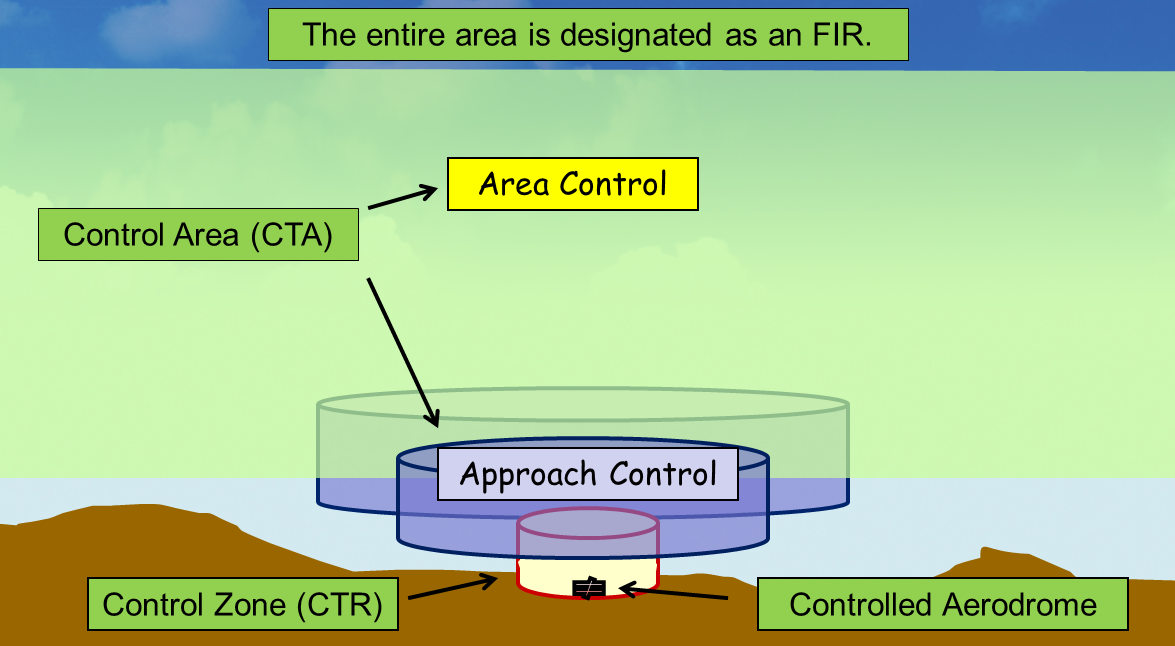
\includegraphics[width=0.9\textwidth]{figures/airspace.png}
    \caption{Airspace division and control \cite[Chapter 2.10]{annex11}}
    \label{fig:airspace}
\end{figure}

\subsection{Air Traffic Control Services}
\subsubsection{Area Control Service}
\subsubsection{Approach Control Service}
\subsubsection{Aerodrome Control Service}
\subsection{Coordination within ATC}
unit $\leftrightarrow$ unit \\
ACC $\leftrightarrow$ APP \\
APP $\leftrightarrow$ TWR \\
sector $\leftrightarrow$ sector

\section{Airspace Classes}
\subsection{Class A}
\subsection{Class B}
\subsection{Class C}
\subsection{Class D}
\subsection{Class E}
\subsection{Class F}
\subsection{Class G}


%poznámky:
%http://en.wikipedia.org/wiki/Controlled\_airspace: rozdíl controlled a uncontrolled: zaveden kvůli vysoké hustotě letů, IFR lety s ATC řízením, bezpečnost
%je v blízkousti vytížených letišť a ve vyšších výškách, kde je cruise, v některých zemích téměř univerzálně, ale zároveň často zachován kus neřízeného prostoru
%třídy A-E

%http://en.wikipedia.org/wiki/Uncontrolled\_airspace neřízený prostor: tam kde to není potřeba nebo není prakticky možné, třídy F a G, ATC neřídí, ale může přes rádio poskytovat informace, typicky VFR lety, mohou být i IFR, ale bez zajištěné separace






% \subsubsection{Area Control Service}
% Area Control Service is an ATC service provided by area control centre (ACC) responsible for flights in Control Areas (CTA). Normally ACC is identified by the name of a nearby city, area or landmark. Smaller countries usually have one ACC, but many larger countries are controlled by several of them. ACCs usually control aircrafts in their en-route phase of flight. The ACC may be also responsible for flights to and from smaller aerodromes with no separate approach control service. \cite[Chapter 3.2]{annex11}
%Control Area contains airways, Terminal Control Areas (TMA) and other airspace. It extends upwards from specified altitude.

% \subsubsection{Approach Control Service}
% Approach Control Service (APP) is ATC service that is responsible for the part of CTA and CTR required by arriving or departing controlled flights (TMA). The primary functions of APP is sequencing arriving aircrafts and assisting departing aircrafts becoming established on course. The arrival and departure functions can be divided into several positions on busy aerodromes. APP is usually identified by the name of the aerodrome which it is serving, but sometimes it's not colocated with TWR and is at distant ACC location. When no separate ACC exists, approach control service is provided by ACC or TWR. \cite[Chapter 3.2]{annex11}

% \subsubsection{Aerodrome Control Service}
% Aerodrome control service is provided by a control tower (TWR) and is responsible for aircraft landing and taking off. It's also responsible for VFR flights in the CTR and for preventing collisions between aircrafts on the manoeuvring are of the aerodrome. \cite[Chapter 3.2]{annex11}

% %\textcolor{red}{z pohledu prostoru/z pohledu kontroly}
% %\textcolor{red}{v každou chvíli řídí letadlo jeden subjekt a místo a čas předání kontroly je jesně definované - kdy a jak?}

% \subsection{Airspace classes}

% %celou kapitolu přepsat, je doslovně  zkopírovaná

% The controlled airspace can furthermore be classified as Class A-G. Classes of airspace are mutually exclusive. Thus, airspace can be Class E and Restricted at the same time, but it cannot be both Class E and Class B at the same location and at the same time. \cite{nolan}

% %On March 12, 1990, ICAO adopted the current airspace classification scheme.[1] The classes are fundamentally defined in terms of flight rules and interactions between aircraft and Air Traffic Control (ATC). Generally speaking, the ICAO airspaces allocate the responsibility for avoiding other aircraft, namely either to ATC (if separation is provided) or to the aircraft commander (if not). definice classes je z annexu 11 - použití v USA z Nolana

% %ICAO adopted classifications
% %Note: These are the ICAO definitions. Country-specific adaptations (such as "two-way communications" instead of "clearance" for Class C in the US) are discussed in the sections below.
% %Class A: All operations must be conducted under IFR. All aircraft are subject to ATC clearance. All flights are separated from each other by ATC.
% %Class B: Operations may be conducted under IFR, SVFR, or VFR. All aircraft are subject to ATC clearance. All flights are separated from each other by ATC.
% %Class C: Operations may be conducted under IFR, SVFR, or VFR. All aircraft are subject to ATC clearance (country-specific variations notwithstanding). Aircraft operating under IFR and SVFR are separated from each other and from flights operating under VFR, but VFR flights are not separated from each other. Flights operating under VFR are given traffic information in respect of other VFR flights.
% %Class D: Operations may be conducted under IFR, SVFR, or VFR. All flights are subject to ATC clearance (country-specific variations notwithstanding). Aircraft operating under IFR and SVFR are separated from each other, and are given traffic information in respect of VFR flights. Flights operating under VFR are given traffic information in respect of all other flights.
% %Class E: Operations may be conducted under IFR, SVFR, or VFR. Aircraft operating under IFR and SVFR are separated from each other, and are subject to ATC clearance. Flights under VFR are not subject to ATC clearance. As far as is practical, traffic information is given to all flights in respect of VFR flights.
% %Class F: Operations may be conducted under IFR or VFR. ATC separation will be provided, so far as practical, to aircraft operating under IFR. Traffic Information may be given as far as is practical in respect of other flights.
% %Class G: Operations may be conducted under IFR or VFR. ATC separation is not provided. Traffic Information may be given as far as is practical in respect of other flights.
% %Classes A–E are referred to as controlled airspace. Classes F and G are uncontrolled airspace.



% Some key concepts are:

% \paragraph{Class A}
% Class A airspace extends from FL180 (18,000 feet (5,500 m) mean sea level MSL) to FL600 (approximately 60,000 feet (18,000 m) MSL) throughout the United States. (AIM 3-2-2) Unlike the altitude measurements used in other airspace classes, the FLnnn flight levels used in Class A airspace are pressure altitudes referenced to a standardized altimeter setting of 29.92" Hg and thus the true altitudes depend on local atmospheric pressure variations.

% Unless otherwise authorized by ATC, all flight operations in Class A airspace must be under ATC control, and must be operating IFR, under a clearance received prior to entry.

% Since Class A airspace is normally restricted to instrument flight only, there are no minimum visibility requirements.

% \paragraph{Class B}
% An example of the Class B Airspace symbol surrounding Denver International Airport.
% Class B airspace is defined around key airport traffic areas, usually airspace surrounding the busiest airports in the US according to the number of IFR operations and passengers served. The exact shape of the airspace varies from one Class B area to another, but in most cases it has the shape of an inverted wedding cake, with a series of circular \"shelves\" of airspace of several thousand feet in thickness centred on a specific airport. Each shelf is larger than the one beneath it. Class B airspace normally begins at the surface in the immediate area of the airport, and successive shelves of greater and greater radius begin at higher and higher altitudes at greater distances from the airport. Many Class B airspaces diverge from this model to accommodate traffic patterns or local topological or other features. The upper limit of Class B airspace is normally 10,000 feet (3,000 m) MSL. (AIM 3-2-3.a.)

% All aircraft entering Class B airspace must obtain ATC clearance prior to entry and must be prepared for denial of clearance. Aircraft must be equipped with a two-way radio for communications with ATC and an operating Mode C transponder, furthermore aircraft overflying the upper limit of any Class B airspace must have an operating Mode C transponder. Visual Flight Rules (VFR) flights may proceed under their own navigation after obtaining clearance but must obey any explicit instructions given by ATC. Some Class B airspaces include special transition routes for VFR flight that require communication with ATC but may not require an explicit clearance. Other Class B airspaces include VFR corridors through which VFR flights may pass without clearance (and without technically entering the Class B airspace). (AIM 3-2-3.b.)

% VFR flights operating in Class B airspace must have three miles (5 km) of visibility and must remain clear of clouds (no minimum distance). (AIM 3-1-4 and 3-2-3.a.)

% Class B airspace has the most stringent rules of all the airspaces in the United States. Class B has strict rules on pilot certification. Pilots operating in Class B airspace must have a private pilot's certificate, or have met the requirement of CFR 61.95. These are often interpreted to mean \"have an instructor's endorsement for having been properly trained in that specific Class B space.\" However, it does not apply to student pilots seeking sport or recreational certificates. Some Class B airports (within Class B airspaces) prohibit student pilots from taking off and landing there and are listed in the AIM section 3-2-3(b)2.

% In addition to this, some Class B airspaces prohibit Special VFR flights.

% Certain Class B airports have a Mode C veil, which encompasses airspace within thirty nautical miles of the airport. Aircraft operating within the Mode C veil must have an operating Mode C transponder (up to 10,000 feet (3,000 m) MSL) unless the aircraft is certified without an engine-driven electrical system and it operates outside the Class B and below the ceiling of the Class B and below 10,000 feet (3,000 m) MSL.

% \paragraph{Class C}
% Class C space is structured in much the same way as Class B airspace, but on a smaller scale. Class C airspace is defined around airports of moderate importance that have an operational control tower and is in effect only during the hours of tower operation at the primary airport. The vertical boundary is usually 4,000 feet (1,200 m) above the airport surface. The core surface area has a radius of five nautical miles (9 km), and goes from the surface to the ceiling of the Class C airspace. The upper \"shelf\" area has a radius of ten nautical miles, and extends from as low as 1,200 feet (370 m) up to the ceiling of the airspace. A procedural Outer Area (not to be confused with the shelf area) has a radius of 20 nautical miles.(AIM 3-2-4)

% All aircraft entering Class C airspace must establish radio communication with ATC prior to entry. The aircraft must be equipped with a two-way radio and an operating Mode C (altitude reporting) radar transponder, furthermore aircraft overflying above the upper limit of Class C airspace upward to 10,000 feet MSL must have an operating Mode C transponder. VFR flights in Class C airspace must have three miles (5 km) of visibility, and fly an altitude at least 500 feet (150 m) below, 1,000 feet (300 m) above, and 2,000 feet (600 m) laterally from clouds. (AIM 3-2-4.c.)

% There is no specific pilot certification required. Aircraft speeds must be below 200 knots (230 mph) at or below 2,500 feet (760 m) above the ground, and within 4 nautical miles (7 km) of the Class C airport. (AIM 3-2-4.c.5.)

% \paragraph{Class D}
% Class D airspace is generally cylindrical in form and normally extends from the surface to 2,500 feet (760 m) above the ground. The outer radius of the airspace is variable, but is generally 4 nautical miles. Airspace within the given radius, but in surrounding Class C or Class B airspace, is excluded. Class D airspace reverts to Class E or G during hours when the tower is closed, or under other special conditions. (AIM 3-2-5)

% Two-way communication with ATC must be established before entering Class D airspace, but no transponder is required. VFR cloud clearance and visibility requirements are the same as Class C. (AIM 3-2-5.b.3)

% \paragraph{Class E}
% Controlled airspace which is neither Class A, B, C nor D. (AIM 3-2-6.a) In most areas of the United States, Class E airspace extends from 1,200 feet (370 m) AGL up to but not including 18,000 feet (5,500 m) MSL, the lower limit of Class A airspace. There are areas where Class E airspace begins at either the surface or 700 AGL, these areas are used to transition between the terminal and en-route environments (around non-towered airports). These areas are designated on sectional charts. Most airspace in the United States is Class E. The airspace above FL600 is also Class E. (AIM 3-2-6.e.7)No ATC clearance or radio communication is required for VFR flight in Class E airspace. VFR visibility and cloud clearance requirements are the same as for Class C and Class D airspaces when below 10,000 feet (3,000 m) MSL. Above 10000 ft MSL, the visibility requirement is extended to 5 miles (8 km) and the cloud clearance requirement is extended to 1,000 feet (300 m) below clouds, 1,000 feet (300 m) above, and 1 mile (1.6 km) laterally. (AIM 3-1-4)

% \paragraph{Class F}
% Class F is not used in the United States.

% \paragraph{Class G}
% Class G airspace includes all airspace below flight level 600 not otherwise classified as controlled. (AIM 3-3-1) There are no entry or clearance requirements for Class G airspace, even for IFR operations. Class G airspace is typically the airspace very near the ground (1200 feet or less), beneath Class E airspace.

% Radio communication is not required in Class G airspace, even for IFR operations. Class G is completely uncontrolled.

% VFR visibility requirements in Class G airspace are 1 mile (1.6 km) by day, and 3 miles (5 km) by night, for altitudes below 10,000 feet (3,050 m) MSL but above 1200 ft AGL. Beginning at 10,000 feet MSL, 5 miles (8 km) of visibility are required, day and night. Cloud clearance requirements are to maintain an altitude that is 500 feet below, 1000 feet above, 2000 horizontal; at or above 10,000 feet MSL, they are 1,000 feet below, 1,000 feet above, and 1 mile laterally. By day at 1,200 feet (370 m) AGL and below, aircraft must remain clear of clouds, and there is no minimum lateral distance.

% It should be noted that there are certain exceptions where Class G extends above 1,200 feet AGL. This is usually either over mountainous terrain (e.g., some areas in the Rocky Mountains), or over very sparsely populated areas (e.g., some parts of Montana and Alaska).

% %The United States also defines categories of airspace that may overlap with classes of airspace. Special use airspace Alert areas Warning areas Restricted airspace Prohibited airspace Military operation area (MOA) Controlled Firing Areas (CFA) National Security Areas (NSA)


% %\textcolor{red}{Pro řízení v terminální oblasti nás zajímají všechny druhy řízení/prostoru, Agentfly má zatím jen ACC v CTA?}

% \begin{figure}[h]
%     \centering
%     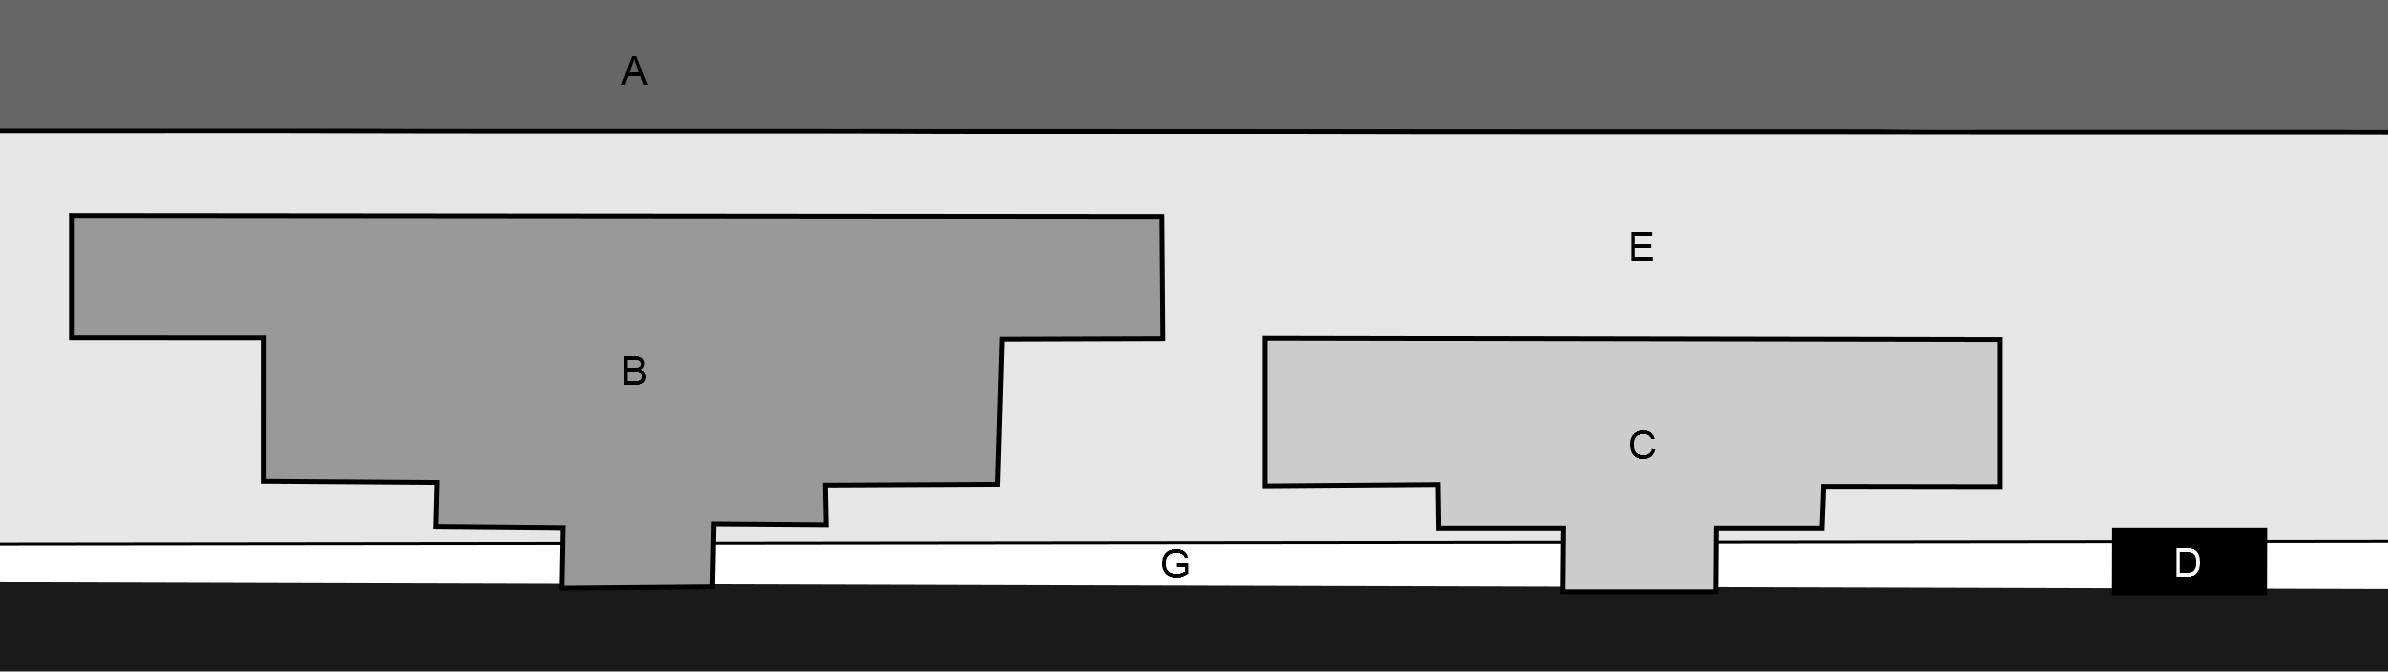
\includegraphics[width=0.8\textwidth]{figures/classes.png}
%     \caption{Airspace Classification - \textcolor{red}{z prezentace 2011 ATM Lesson Plans/ATM 1-2 General Air Traffic Control Service \cite {nolan}% - překreslit!
%     }}
%     \label{fig:classes}
% \end{figure}

% \begin{figure}[h]
%     \centering
%     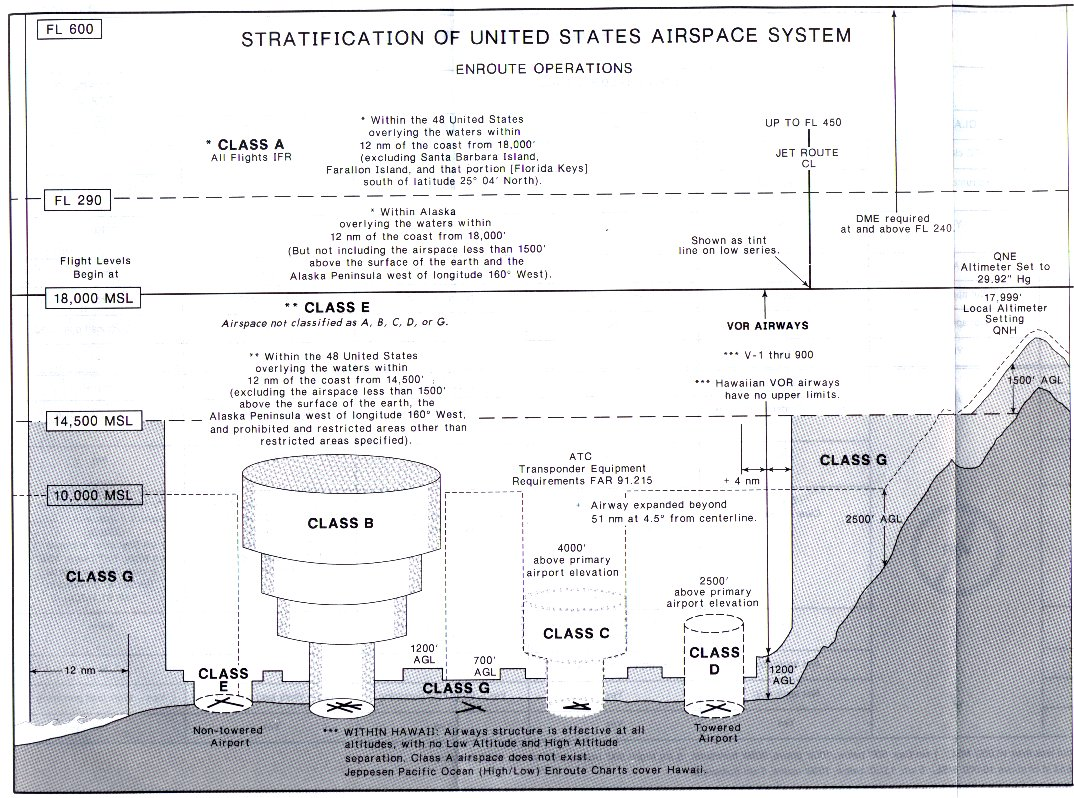
\includegraphics[width=\textwidth]{figures/classes2.jpg}
%     \caption{Airspace Classification - http://m1heli.com/helicopter\%20pictures/airclass.jpg}
%     \label{fig:classes2}
% \end{figure}

% %\textcolor{red}{SID a STAR routy?}

% \subsubsection{Airspace Management}
% ATM is generic term for any management activity for achieving the most eficient and flexible use of airspace avoiding permanent airspace segregation. %\textcolor{red}{zdroj jen z prezentace}
% The goals are to improve coordination between civil and military agencies, optimise route network and airspace structure and develop a free route airspace concept.

% The concept of Flexible Use of Airspace (FUA) means that airspace should be treated as one continuous space that is being allocated according to user requirements. Any airspace segregation should only be temporary.

% \subsubsection{Coordination within ATC}
% unit $\leftrightarrow$ unit \\
% ACC $\leftrightarrow$ APP \\
% APP $\leftrightarrow$ TWR \\
% sector $\leftrightarrow$ sector \\
% sectors are within units

% koordinaci mezi sektory popisuje \cite{doc4444} Doc 4444 Chapter 10
% Detailed procedures are often subject to local regulations and rules.

% Transferring unit/controller transfers the responsibility to control the aircraft to the accepting unit on point of transfer of control.

% The transfer of control can be divided into three stages. First the flight is \bold{notified} to prepare for the transfer. Then the conditions of transfer of control are \bold{negotiated} with the transferring ATC unit and if necessary also with the accepting unit. After the parties \bold{agree}, the control is transferred to the accepting unit. his process can be achieved using automated means (AFTN, RDPS, FDPS, OLDI \textcolor{red}{?}) without using conventional telephone coordination. %\textcolor{red}{(Jakože mezi sektory, s letadlem domluva asi pořád probíhá.)} 
% \cite[Chapter 10.1.1]{doc4444}

% This means that the flight is at any time under the control of only one ATC unit and can't be transferred from one unit to another without consent of the accepting unit. Also if communication with the aircraft is transwerred to the next unit, that unit cannot change the learance of the aircraft before the point of control transfer.

% %Doslovně z prezentace:
% Control of an aircraft shall be transferred from ACC to APP, and vice versa, at a time or point agreed between the two units. This time or point is normally stated in a LOA.
% Except when otherwise specified, APP may issue clearances to any aircraft released to it by ACC without reference to ACC. If an aircraft executes a missed approach, if necessary, ACC shall be informed immediately and subsequent action coordinated. 
% After coordination with APP, ACC may release an arriving aircraft directly to TWR if the entire approach will be made under VMC.\cite[Chapter 10.1.3.1]{doc4444}

% %Doslovně z prezentace:
% The take-off time is specified by the ACC when it needs to coordinate the departure with other ACC traffic or provide separation between other departing traffic on the same track. In other cases the APP determines the time of take-off so that the traffic in their AOR is separated. ACC and APP can also specify clearance expiry time if a delayed departure would cause separation problems. The time given by APP must not be later than ACC time. co je AOR?\cite[Chapter 10.1.3.2]{doc4444}

% %Doslovně z prezentace:
% Exchange of movement and control data
% APP shall keep ACC advised of data about controlled traffic such as:
% RWY in use and type of instrument approach procedure;
% lowest available level at the holding fix for use by ACC;
% average time or distance intervals between successive arrivals as determined by APP;
% revision of EATs as required (5 MIN or greater, or as agreed);
% arrival times over holding fix when these vary by 3 MIN or greater from the times estimated by ACC;
% flights cancelling IFR, if it will affect holding levels or EATs;
% departure times, or if agreed, boundary or specified point times;
% information relating to overdue or unreported aircraft; and
% missed approach times which may affect ACC.
% \cite[Chapter 10.1.3.3]{doc4444}

% %Doslovně z prezentace:
% ACC shall keep APP advised of data about controlled traffic such as:
% identification, type and point of departure of arrivals;
% ETA and level of arrivals over holding fix or other specified point;
% ATA and level of arrivals over holding fix if aircraft is released to APP after arriving over the holding fix;
% requested type of instrument approach procedure if different to that specified by APP;
% EAT issued;
% when required, that an aircraft has been instructed to contact APP;
% when required, that an aircraft has been released to APP, including if necessary, the time and conditions of release; and
% anticipated delay to departures due to congestion.
% ACC shall forward information on arrivals at least 15 MIN before ETA. \cite[Chapter 10.1.3.3]{doc4444}

% %Doslovně z prezentace:
% Division of control
% APP shall retain control of arrivals until the aircraft have been transferred to, and are in communication with TWR. Rules for transfer of control of arrivals shall be establish by LOAs or local instructions, considering airspace structure, terrain, MET conditions and ATS facilities available.
% APP may authorize TWR to release a departure for take-off subject to the discretion of TWR with respect to arrivals.
% TWR shall obtain approval from APP prior to authorizing SVFR flights, when so prescribed in LOAs or local instructions. \cite[Chapter 10.1.4.1]{doc4444}

% %Doslovně z prezentace:
% Exchange of movement and control data
% TWR shall keep APP advised of data about controlled traffic such as:
% \bitem
% \item arrival and departure times;
% \item when required, that the first aircraft in the approach sequence is in  	communication with and is sighted by TWR, and that reasonable 	assurance exists that a landing will be accomplished;
% \item information relating to overdue or unreported aircraft;
% \item information concerning missed approaches; and
% \item information concerning aircraft that are essential local traffic to aircraft 	under the control of APP.
% \eitem
% \cite[Chapter 10.1.4.2]{doc4444}

% %Doslovně z prezentace:
% Transfer of control
% For arriving aircraft control shall be transferred from APP to TWR when the aircraft:
% \bitem
% \item is in the vicinity of the aerodrome, and
% 	\bitem
% 	\item it is considered that approach and landing will be completed in visual reference to the ground, or
% 	\item has reached uninterrupted VMC; or
% 	\eitem
% \item is at a prescribed point or level; or
% \item has landed, 
% 	as specified in LOAs or unit instructions.
% \eitem
% Transfer of communication to TWR should at a point, level or time that landing clearance, alternative instructions and essential local traffic information can be issued in a timely manner.

% For departing aircraft control shall be transferred from TWR to APP:
% \bitem
% \item when VMC prevail in the vicinity of the aerodrome:
% 	\bitem
% 	\item prior to the time the aircraft leaves the vicinity of the aerodrome;
% 	\item prior to the aircraft entering IMC; or
% 	\item when the aircraft is at a prescribed point or level, as specified in LOAs or unit instructions; 
% 	\eitem
% \item when IMC prevail at the aerodrome:
% 	\bitem
% 	\item immediately after the aircraft is airborne; or
% 	\item when the aircraft is at a prescribed point or level, as specified in LOAs or unit instructions.
% 	\eitem
% \eitem
% \cite[Chapter 4.3.2]{doc4444}

% Control shall be transferred from one sector/position to another within the same ATC unit at a point, level or time, as specified in local instructions.
% FPL and control information shall be exchanged between control positions within the same unit, in respect of:
%   all aircraft for which control will be transferred from one unit to another;
%   aircraft operating in such close proximity to an adjacent sector boundary 	that control of traffic in that sector may be affected;
%   all aircraft for which control will be transferred from a procedural controller 	to a surveillance controller, as well as other aircraft affected.
% These transfer of control and coordination procedures shall conform to agreements applicable to the ATC units.
% Even with all the modern electronic equipment and highly developed systems, coordination between controllers within a single sector, or adjoining sectors, if often based on clear, simple conversation. 
% This conversation is often conducted in the local native language or, when controllers are busy and occupied with other responsibilities, this communication may be conducted using body language (e.g. raising a hand or nodding the head). 
% Such coordination is normally not specified in local rules, and it important that controllers are very careful to ensure there is no misunderstanding between them.
% \cite[Chapter 4.3.5, 10.1.5]{doc4444}

% ICAO requires that a flight plan (FPL) message containing basic flight plan data is forwarded to the first ACC at least 30 minutes in advance of the flight, and to successive ACCs at least 20 minutes in advance of the flight reaching their area. Normally, due to flow control procedures and general air traffic planning requirements, this minimum is increased to 1 hour or even more, depending on agreements between units. 
% If ATC clearances change the route of flight so the aircraft will fly through other ATC areas of responsibility, a current flight plan (CPL) message must be forwarded to those units at least 20 minutes prior to entering their area. Normally, agreements between units will specify an increased time.
% An estimate (EST) message shall be forwarded at least 20 minutes prior to a flight entering a unit’s area of responsibility. This message contains the essential control information such as estimate, level and SSR code. The 20 minute time period may be increased or decreased, based on unit requirements and agreements.
% \cite[Chapter 11.3,4]{doc4444}

% Most common types of ATC coordination:
% \bitem
% \item current flight plan (20 MIN or more prior to control boundary) 
% \item estimate (20 MIN prior to control boundary, or LOAs); 
% \item revision (no ICAO defined time, LOAs);
% \item approval request (no ICAO defined time, LOAs); and
% \item transfer of control.
% \eitem

%!TEX root = index.tex

\section{Flight Plan}

Every controlled aircraft has its flight plan (FP) that contains basic information about the flight. These information include aircraft identification, aircraft type, departure point, departure time, route of flight, destination, fuel on board and a few other. \cite[Chapter 5]{aim} The purpose of the flight plan is to give all relevant data about the aircraft to the air traffic controller in a standardized format so it can be used efficiently during the flight control. The flight plan is handed over from one control to another as the aircraft progresses from its departure airport to destination along the flight route.

The flight route is a sequence of fixes and routes the plane will fly through during its flight.

\subsection{Fix}
Fix is named point on Earth that aircraft use for their navigation. The position of fix can be determined by radio beacons or as GPS position for airplanes equipped with GPS receivers.

If aircraft has certain fix in its flight plan, it must fly over the position of the fix during the flight. This way the route of the aircraft is defined and automatic tools can be used to notify the pilot and air traffic controller if the plane deflects too far from the trajectory defined by its flight plan.

\subsection{Route}
Route is named sequence of fixes. There can be some additional restrictions added on the route, for example altitude at given fixes or type of aircraft that can use the route. The flight plan does not need to include the whole route, the plane can be ordered to follow only part of the route between two fixes.

\subsubsection{STAR}
Standard instrument arrival (STAR). A designated instrument flight rule (IFR) arrival route linking a significant point,
normally on an ATS route, with a point from which a published instrument approach procedure can be commenced. \cite{doc4444}

\subsubsection{SID}
Standard instrument departure (SID). A designated instrument flight rule (IFR) departure route linking the aerodrome
or a specified runway of the aerodrome with a specified significant point, normally on a designated ATS route, at
which the en-route phase of a flight commences



%\section{Airports}
%\subsection{Ground}

\section{Used Units}
\subsection{Altimetry}

% \subsection{Altimetry}
% Výška nad mořem/terénem/tlak/potřeba referenční hladiny, závisí na teplotě=tlaku vzduchu

% QNE - standardní nastavení - letí se podle flight levelů - výška od referenční hladiny 1013.2 hPa
% QNH - letí se podle nadmořské výšky, je to hodnota tlaku na daném místě (typicky letišti) který po zadaání do výškoměru vrací správnou nadmořskou výšku
% QFE - výška nad povrchem země v daném místě - typicky u letiště


% Transition altitude
% The TA is the altitude at or below which the vertical position is expressed in terms of altitudes. The TA is established by the appropriate ATS authority.

% Transition level (TL) is flight level just above the TA. Transition layer is the layer between TA and TL. It is prohibited to fly on the level that is in the transition layer.

% When the plane is descending the pilot changes from QNE to QNH when passing TL. When climbing pilot changes from QNH to QNE on TA.

% Řídící musí včas předat letadlu hodnotu QNH a TL.

\section{Separation}

Along with transferring control over aircraft from one sector to another and applying standard operating procedures for take-off or landing is keeping air traffic separated one of the main duties of air traffic controller. Proper separation ensures security and eliminates risk of collision. \cite[Chapter 2]{order7110}

Vertical or horizontal separation must be provided for all flights in Class A and B airspaces, IFR flights in Class C, D and E airspaces and between IFR and VFR flights in Class C airspace. \cite[Chapter 5]{doc4444}

The rules air traffic controllers use to keep aircraft separated are called separation minima. Separation can be achieved in two basic ways: vertical and horizontal. Their description follows.

\subsection{Vertical}

Vertical separation is reached when ATC controller assigns planes different cruising levels. Historically vertical separation minima were set to 1000 ft (10FL) below FL290 and 2000 ft above FL290. This was due to the fact that altimeter precision decreases with increasing altitude. Over time more precise altimeters and combination with other means of measuring aircraft altitude allowed to decrease the 2000 ft separation minima and introduce the Reduced vertical separation minima (RVSM) system. In the RVSM airspace the separation limit is 1000 ft up to FL410 and 2000 ft above this level. If the cruising altitude of two airplanes is greater or equal as the separation minima, the airplanes are considered as separated. \cite{aim}

Other rules can be applied, often different flight levels are reserved for aircraft flying in certain direction. Example of such rule can be that eastbound flights (with heading 0$^{\circ}$ – 179$^{\circ}$) fly on even tenths flight levels (FL20, FL40 etc.) and westbound flights (with heading 180$^{\circ}$ – 359$^{\circ}$) fly on odd tenths (FL10, FL30 etc.).


\subsection{Horizontal}
\subsubsection{Longitudinal}
\subsubsection{Lateral}

% \item horizontal
% 	\bitem
% 	\item longitudinal - interval between planes flying on the same (converging, reciprocal) is maintained
% 	\item lateral - planes fly on different routes
% 	\eitem
% \item composite - combination of the above
% \eitem
% \cite[Chapter 3.3]{doc4444}



% \subsubsection{Longitudinal}
% 15/10/5 minut separace nad stejným bodem podle typu situace 
% \cite[Chapter 5.4.2.2]{doc4444}


% \subsubsection{Minima (for procedural control?)}
% For arriving MEDIUM aircraft after HEAVY: 2 minutes. LIGHT after HEAVY 3 minutes. \cite[Chapter 5.8.2]{doc4444}
% For departing LIGHT or MEDIUM aircraft after HEAVY: 2 minutes. LIGHT after MEDIUM 2 minutes. \cite[Chapter 5.8.3]{doc4444}
% %A DALŠÍ VARIANTY... viz prezentace

% \subsubsection{Minima (for surveillance control?)}
% \bitem
% \item Heavy - 136 tonne or more
% \item Medium - 7-136 tonne
% \item Light - 7 tonne or less
% \eitem
% For both arrival and departure of planes provided with surveillance service: (also enroute at the same altitude or less than 1000ft below or parallel runway separated by less than 2500ft)
% \bitem
% \item H after H: 4NM
% \item M after H: 5NM
% \item L after H: 6NM
% \item L after M: 5NM
% \eitem
% \cite[Chapter 8.7.3]{doc4444}

\subsection{Wake Turbulence Separation}

Wake turbulence is the air vortex formed behind every aircraft as it moves through the air. The strength and size of the vortex depends on the parameters of the aircraft (mass, size, speed, wing configuration, etc.). It's not visible and can cause hazardous situation for the following aircraft especially if it is smaller and lighter and therefore more susceptible to be affected by the vortex.

Special alertness is needed in conditions with light wind, because the turbulence won't dissipate quickly and may drift to parallel runway or descend to lower altitude into path of following aircraft.

\red{TODO}

\section{Holding}

Holding procedure is a predefined manoeuvre that keeps the aircraft in predetermined airspace while waiting for clearance. The procedure is the same for VFR and IFR flights. Holding fix is a geographical location that serves as a reference point for holding procedure. The pattern itself is defined by the holding fix, heading of the inbound leg and length of the pattern. \cite[Chapter 6]{doc4444} The pattern and some terms used for it's description are shown in Figure \ref{fig:holding}.

Reasons for holding can be traffic congestion, delays at destination airport or aircraft problems.

\red{TODO}

\begin{figure}[h]
    \centering
    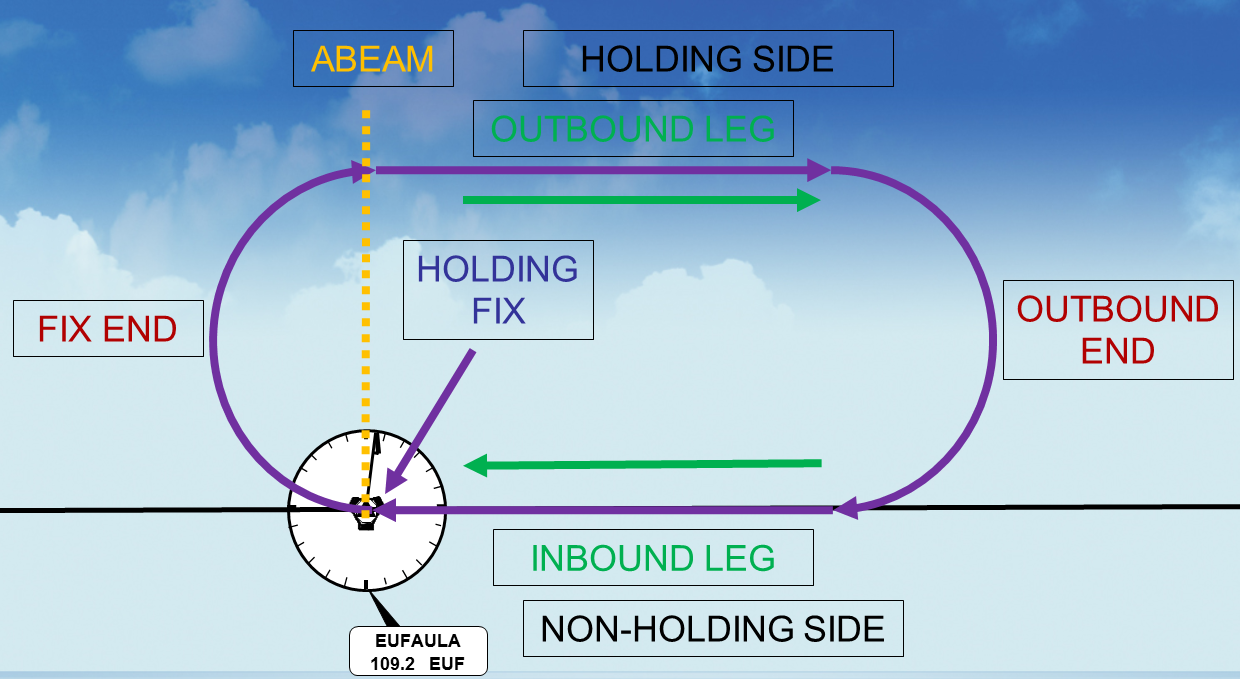
\includegraphics[width=0.9\textwidth]{figures/holding.png}
    \caption{Holding pattern with examples of entry}
    \label{fig:holding}
\end{figure}
% %Doplnit popis jednotlivých entry procedures!

% If the delay is expected, the aircraft should be notified as soon as possible and if practical advised to reduce speed in order to absorb the delay. The ACC is normally responsible for clearing the aircraft to the holding fix including the instruction for the holding procedure itself and EAT.\\
% The holding procedure (including the pattern etc.) is normally published beforehand. Otherwise ATC shall specify the details of the procedure. Normally the first arriving aircraft is at the lovest level and the following aircrafts at successively higher levels. Turbojet aircrafts can be held at higher levels in order to conserve fuel, but ther order must be retained.\\
% Vertical separation is mantained amongst the aircrafts in the holding sequence. Vertical separation must be applied whenever other aircraft is within 5 minutes of the holding area.\cite[Chapter 6.5.5]{doc4444}

% The EAT should be established for aircrafts expected to be delayed for 10 minutes or more and transmitted to the aircraft as soon as practicable. It should be retransmitted if the updated EAT differs from the previous time by 5 minutes or more.\cite[Chapter 6.5.7]{doc4444}

% \subsection{Hartsfield–Jackson Atlanta International Airport}
% Hartsfield–Jackson Atlanta International Airport (ICAO code KATL) has been the world's busiest airport by passenger traffic since 1998 with more than 94 million passengers in 2013. It has also the most landings and take-offs since 2005. The airport has 207 domestic and international gates which is the most at any airport. \cite{atlanta}
%  Proč zvolena pro testy Atlanta...


\section{Miles In Trails}